\documentclass[11pt]{beamer}
\usepackage{tcolorbox}
% Required packages
\usepackage{booktabs}
\usepackage{amsmath}
\usepackage{capt-of} % instead of caption
\usepackage{multicol}
\usepackage[siunitx]{circuitikz} 
\usetikzlibrary{shapes.geometric}
% or \bibliographystyle{plainnat} % Alternative style
% Theme settings
\usetheme{Boadilla}
\useinnertheme{circles}
\useoutertheme{miniframes}
\setbeamertemplate{navigation symbols}{}


% Colors
\definecolor{primaryColor}{RGB}{20,45,105}
\definecolor{secondaryColor}{RGB}{0,100,160}

\setbeamercolor{structure}{fg=primaryColor}
\setbeamercolor{palette primary}{bg=primaryColor, fg=white}
\setbeamercolor{palette secondary}{bg=secondaryColor, fg=white}
\setbeamercolor{title}{bg=primaryColor, fg=white}
\setbeamercolor{headline}{bg=secondaryColor, fg=white}
\setbeamercolor{section in head/foot}{bg=primaryColor, fg=white}
\setbeamercolor{subsection in head/foot}{bg=secondaryColor, fg=white}
\setbeamercolor{author in head/foot}{bg=primaryColor, fg=white}
\setbeamercolor{title in head/foot}{bg=secondaryColor, fg=white}
\setbeamercolor{date in head/foot}{bg=primaryColor, fg=white}
\setbeamercolor{page number in head/foot}{bg=primaryColor, fg=white}

% Presentation metadata
\title[EN2091 Laboratory Practice \& Projects]{Five Band Audio Equalizer}
\author[Electro Dieus]{\texorpdfstring{Disssanayake R.K.T.(230164K)\\Ratnayake R.M.S.H.(230548R)\\Shehan M.N.N.(230613M)\\Tennakoon U.G.R.B.(230629R)}{Disssanayake R.K.T., Ratnayake R.M.S.H., Shehan M.N.N., Tennakoon U.G.R.B.}}
\institute[]{Department of Electronic \& Telecommunication Engineering\\ University of Moratuwa, Sri Lanka}
\date{December 11, 2025}

% Document starts here
\begin{document}
	
	\begin{frame}
		\titlepage
	\end{frame}
	
	\begin{frame}
		\frametitle{Presentation Structure}
		\tableofcontents
	\end{frame}
	
	
	\section{Introduction}
	\begin{frame}
		\begin{center}
			{\Huge Introduction}
		\end{center}
	\end{frame}
	\begin{frame}{System Architecture}
		\centering
		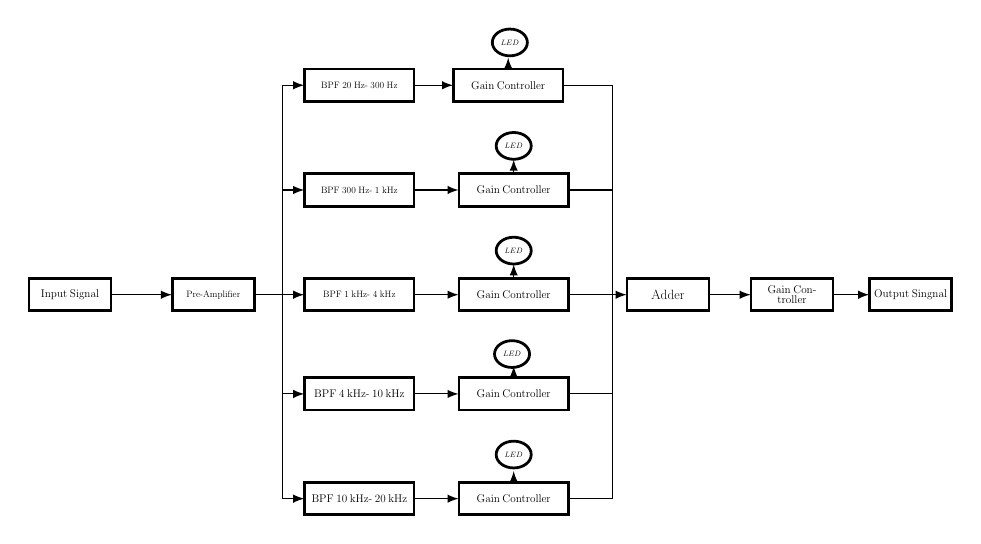
\begin{tikzpicture}[scale=0.28,transform shape]	% Paths, nodes and wires:
			\node[shape=rectangle, draw, line width=1pt, minimum width=3.715cm, minimum height=1.465cm] at (-26.625, 11.75){} node[anchor=center, align=center, text width=3.327cm, inner sep=6pt] at (-26.625, 11.75){\Large Input Signal};
			\node[shape=rectangle, draw, line width=1pt, minimum width=3.715cm, minimum height=1.465cm] at (-20.125, 11.75){} node[anchor=center, align=center, text width=3.327cm, inner sep=6pt] at (-20.125, 11.75){\large Pre-Amplifier};
			\node[shape=rectangle, draw, line width=1pt, minimum width=4.965cm, minimum height=1.465cm] at (-13.5, 21.25){} node[anchor=center, align=center, text width=4.577cm, inner sep=6pt] at (-13.5, 21.25){\large BPF 20 Hz- 300 Hz};
			\node[shape=rectangle, draw, line width=1pt, minimum width=4.965cm, minimum height=1.465cm] at (-13.5, 11.75){} node[anchor=center, align=center, text width=4.577cm, inner sep=6pt] at (-13.5, 11.75){\large BPF 1 kHz- 4 kHz};
			\node[shape=rectangle, draw, line width=1pt, minimum width=4.965cm, minimum height=1.465cm] at (-13.5, 16.5){} node[anchor=center, align=center, text width=4.577cm, inner sep=6pt] at (-13.5, 16.5){\large BPF 300 Hz- 1 kHz};
			\node[shape=rectangle, draw, line width=1pt, minimum width=4.965cm, minimum height=1.465cm] at (-13.5, 7.25){} node[anchor=center, align=center, text width=4.577cm, inner sep=6pt] at (-13.5, 7.25){\Large BPF 4 kHz- 10 kHz};
			\node[shape=rectangle, draw, line width=1pt, minimum width=4.965cm, minimum height=1.465cm] at (-13.5, 2.5){} node[anchor=center, align=center, text width=4.577cm, inner sep=6pt] at (-13.5, 2.5){\Large BPF 10 kHz- 20 kHz};
			\node[shape=rectangle, draw, line width=1pt, minimum width=4.965cm, minimum height=1.465cm] at (-6.75, 21.25){} node[anchor=center, align=center, text width=4.577cm, inner sep=6pt] at (-6.75, 21.25){\Large Gain Controller};
			\node[shape=rectangle, draw, line width=1pt, minimum width=4.965cm, minimum height=1.465cm] at (-6.5, 16.5){} node[anchor=center, align=center, text width=4.577cm, inner sep=6pt] at (-6.5, 16.5){\Large Gain Controller};
			\node[shape=rectangle, draw, line width=1pt, minimum width=4.965cm, minimum height=1.465cm] at (-6.5, 11.75){} node[anchor=center, align=center, text width=4.577cm, inner sep=6pt] at (-6.5, 11.75){\Large Gain Controller};
			\node[shape=rectangle, draw, line width=1pt, minimum width=4.965cm, minimum height=1.465cm] at (-6.5, 7.25){} node[anchor=center, align=center, text width=4.577cm, inner sep=6pt] at (-6.5, 7.25){\Large Gain Controller};
			\node[shape=rectangle, draw, line width=1pt, minimum width=4.965cm, minimum height=1.465cm] at (-6.5, 2.5){} node[anchor=center, align=center, text width=4.577cm, inner sep=6pt] at (-6.5, 2.5){\Large Gain Controller};
			\node[shape=rectangle, draw, line width=1pt, minimum width=3.715cm, minimum height=1.465cm] at (0.5, 11.75){} node[anchor=center, align=center, text width=3.327cm, inner sep=6pt] at (0.5, 11.75){\LARGE Adder};
			\node[shape=rectangle, draw, line width=1pt, minimum width=3.715cm, minimum height=1.465cm] at (6.125, 11.75){} node[anchor=center, align=center, text width=3.327cm, inner sep=6pt] at (6.125, 11.75){\Large Gain Controller};
			\node[shape=rectangle, draw, line width=1pt, minimum width=3.715cm, minimum height=1.465cm] at (11.5, 11.75){} node[anchor=center, align=center, text width=3.327cm, inner sep=6pt] at (11.5, 11.75){\Large Output Singnal};
			\node[shape=ellipse, draw, line width=1pt, minimum width=1.59cm, minimum height=1.215cm](N1) at (-6.675, 23.192){} node[anchor=center] at (N1.text){$LED$};
			\node[shape=ellipse, draw, line width=1pt, minimum width=1.59cm, minimum height=1.215cm](N2) at (-6.5, 18.5){} node[anchor=center] at (N2.text){$LED$};
			\node[shape=ellipse, draw, line width=1pt, minimum width=1.59cm, minimum height=1.215cm](N3) at (-6.5, 13.75){} node[anchor=center] at (N3.text){$LED$};
			\node[shape=ellipse, draw, line width=1pt, minimum width=1.59cm, minimum height=1.215cm](N4) at (-6.575, 9.058){} node[anchor=center] at (N4.text){$LED$};
			\node[shape=ellipse, draw, line width=1pt, minimum width=1.59cm, minimum height=1.215cm](N5) at (-6.5, 4.5){} node[anchor=center] at (N5.text){$LED$};
			\draw[-latex] (-24.75, 11.75) -- (-22, 11.75);
			\draw[-latex] (-18.25, 11.75) -- (-16, 11.75);
			\draw[-latex] (-17, 11.75) -- (-17, 7.25) -- (-16, 7.25);
			\draw[-latex] (-17, 7.25) -- (-17, 2.5) -- (-16, 2.5);
			\draw[-latex] (-17, 11.75) -- (-17, 16.5) -- (-16, 16.5);
			\draw[-latex] (-17, 16.5) -- (-17, 21.25) -- (-16, 21.25);
			\draw[-latex] (-11, 21.25) -- (-9.25, 21.25);
			\draw[-latex] (-11, 16.5) -- (-9, 16.5);
			\draw[-latex] (-11, 11.75) -- (-9, 11.75);
			\draw[-latex] (-11, 7.25) -- (-9, 7.25);
			\draw[-latex] (-11, 2.5) -- (-9, 2.5);
			\draw[-latex] (-6.5, 3.25) -- (-6.5, 3.75);
			\draw[-latex] (-6.5, 8) -- (-6.5, 8.5);
			\draw[-latex] (-6.5, 12.5) -- (-6.5, 13.125);
			\draw[-latex] (-6.5, 17.25) -- (-6.5, 17.75) -- (-6.5, 17.875);
			\draw[-latex] (-6.75, 22) -- (-6.75, 22.5);
			\draw[-latex] (-4, 11.75) -- (-1.375, 11.75);
			\draw[-latex] (2.375, 11.75) -- (4.25, 11.75);
			\draw[-latex] (8, 11.75) -- (9.625, 11.75);
			\draw (-4, 2.5) -- (-2, 2.5) -- (-2, 11.75);
			\draw (-4, 7.25) -- (-2, 7.25);
			\draw (-4.25, 21.25) -- (-2, 21.25) -- (-2, 11.75);
			\draw (-4, 16.5) -- (-2, 16.5);
		\end{tikzpicture}
		
	\end{frame}
	\begin{frame}{Component Selection Justification}
		\centering
		\begin{enumerate}
			\item\textbf{NE5532 Operational Amplifier}
			\begin{itemize}
				
				\item \textbf{Low Noise}: 5\,nV/$\sqrt{\text{Hz}}$ suitable for high-fidelity audio
				\item \textbf{Bipolar Input}: Ensures low offset and distortion in precision audio
				\item \textbf{Dual Channel}: Two op-amps per IC for compact design
				\item \textbf{High Slew Rate}: 9\,V/$\mu$s supports wide dynamic range
				\item \textbf{Wide Bandwidth}: 10\,MHz gain-bandwidth product for audio applications
				\item \textbf{Wide Supply}: $\pm3$\,V to $\pm20$\,V operation for design flexibility
				\item \textbf{High Drive Capability}: Can directly drive 600\,$\Omega$ loads
			\end{itemize}
			
			
			\item \textbf{LM3915 Dot/Bar Display Driver}
			\begin{itemize}
				\item Logarithmic 3 dB/step response for audio
				\item Direct LED drive without current-limiting resistors
				\item Simple setup with minimal external components
				\item Over-voltage protection ($\pm$35V) on input
			\end{itemize}
			
			
		\end{enumerate}
	\end{frame}
	
	
	\begin{frame}{Component Selection Justification (Contd..)}
		\begin{minipage}[t]{0.48\textwidth}
			\centering
			\includegraphics[width=0.8\textwidth]{images.jpeg}
			\captionof{figure}{NE5532 Operational Amplifier}
		\end{minipage}
		\hfill
		\begin{minipage}[t]{0.48\textwidth}
			\centering
			\includegraphics[width=1\textwidth]{lm3914.png}
			\captionof{figure}{LM3915 Dot/Bar Display Driver}
		\end{minipage}
	\end{frame}
	
	
	
	\section{PCB Design}
	\begin{frame}
		\begin{center}
			{\Huge PCB Design}
		\end{center}
	\end{frame}
	
	\begin{frame}{PCB 2D Pathways}
		\centering
		
		\begin{multicols}{2}
			\begin{figure}[H]
				\centering
				\includegraphics[width=\linewidth]{pre}
				\caption{Pre-Amplifier Circuit}
				\label{fig:preamp}
			\end{figure}
			\begin{figure}[H]
				\centering
				\includegraphics[width=\linewidth]{pow.png}
				\caption{Power Amplifier}
				\label{fig:powamp}
			\end{figure}
		\end{multicols}
	\end{frame}
	
	\begin{frame}{PCB 2D Pathways (Contd...)}
		\centering
		
		\begin{multicols}{2}
			\begin{figure}[H]
				\centering
				\includegraphics[width=\linewidth]{fil.png}
				\caption{Filters}
				\label{fig:filters}
			\end{figure}
			\begin{figure}[H]
				\centering
				\includegraphics[width=\linewidth]{display.png}
				\caption{LED Display}
				\label{fig:display}
			\end{figure}
		\end{multicols}
	\end{frame}
	% Add this in your presentation after the initial PCB Design slide
	
	\begin{frame}{PCB Partitioning: A Cost-Effective Approach}
		
		\begin{block}{Initial Design: 2 PCBs}
			\begin{itemize}
				\item \textbf{Main Circuit PCB:} 162.94 mm $\times$ 112.52 mm
				\item  \textbf{Display PCB:} 119.63 mm $\times$ 58.67 mm
				\item \textbf{Total Estimated Cost:} $\approx $\textbf{\$20}
			\end{itemize}
		\end{block}
		
		\begin{block}{Final Design: 4 PCBs}
			\begin{itemize}
				\item Four smaller, modular boards, each under \textbf{100 mm $\times$ 100 mm}
				\item Standard size qualifying for low-cost prototyping services
				\item \textbf{Total Cost:} 4 boards $\times$ \$2 = \textbf{\$8}
			\end{itemize}
		\end{block}
		
		\begin{exampleblock}{Key Outcome: 60\% Cost Reduction}
			 By splitting the design into four smaller, standardized panels, we achieved a significant \textbf{60\% reduction in manufacturing cost} without compromising system functionality or performance.
		\end{exampleblock}
		
	\end{frame}
	\begin{frame}{PCB Testing}
    			
			\begin{center}
			
			% Use the same image as thumbnail
			\includegraphics[width=0.6\linewidth]{hardware2.jpg}
			
			\vspace{0.5cm}
			
			% Clickable link that actually works
			\href{run:pcb.mp4}{
				\fcolorbox{blue}{white}{
					\textcolor{blue}{\Large\textbf{Click to Play Video}}
				}
			}
			
		\end{center}
	    
	\end{frame}
    
	\section{Enclosure Design}
	\begin{frame}
		\begin{center}
			{\Huge Enclosure Design}
		\end{center}
	\end{frame}
	\begin{frame}{Enclosure Design}
\begin{center} % Use the same image as thumbnail 
\includegraphics[width=\linewidth]{Project_analog_3-0004.png} 
\vspace{0.5cm} % Clickable link that actually works 
\href{run:enclosure.mp4}{ \fcolorbox{blue}{white}{ \textcolor{blue}{\Large\textbf{Click to Play Video}} } } 
\end{center}


	\end{frame}
    \begin{frame}{Final Product}
        \begin{figure}
            \centering
            \includegraphics[width=0.7\linewidth]{Final.png}
            \caption{Five Band Audio Equalizer }
            \label{fig:placeholder}
        \end{figure}
    \end{frame}
	\section{Conclusion}
	
		\begin{frame}
		\begin{center}
			{\Huge  Conclusion}
		\end{center}
	\end{frame}
	\begin{frame}{Technical Challenges \& Solutions}
		
		
		
		\begin{exampleblock}{Op-Amp Signal Distortion}
			\begin{itemize}
				\item \textbf{Problem:} TL072 op-amps caused severe distortion at high frequencies
				\item \textbf{Solution:} Upgraded to NE5532 for better slew rate and bandwidth
				\item \textbf{Result:} Clean signal across all frequency bands
			\end{itemize}
		\end{exampleblock}
		
		\begin{exampleblock}{Filter Component Mismatch}
			\begin{itemize}
				\item \textbf{Problem:} Theoretical resistor values didn't match practical performance
				\item \textbf{Solution:} Recalculated values and verified -3 dB points with oscilloscope
				\item \textbf{Result:} Precisely tuned filters meeting all specifications
			\end{itemize}
		\end{exampleblock}

		
	\end{frame}
	\begin{frame}{Contribution of Group Members}
\centering
\renewcommand{\arraystretch}{0.9} % Adjust line height slightly
\begin{tabular}{|l|p{6cm}|} % p{6cm} allows auto line wrapping
\hline
\textbf{Student's Name (Index No.)} & \textbf{Contribution} \\
\hline
Tennakoon U.G.R.B. (230629R) & Filter calculations, PCB design, Testing \& debugging, Soldering \\
\hline
Ratnayake R.M.S.H. (203548R) & PCB design, Circuits design, Circuits simulation, Soldering \\
\hline
Shehan M.N.N. (230613M) & Breadboard implementation, Enclosure Design, Testing \\
\hline
Dissanayake R.K.T. (230164K) & LED display circuit design \& breadboard implementation, Testing, Assembling \\
\hline
\end{tabular}
	\end{frame}

    
	\begin{frame}
		\begin{center}
			{\Huge Thank You!}
		\end{center}
	\end{frame}
	
\end{document}
